
% ********** Chapter 6 **********
\chapter{SIP Call Component}
\label{sec:SIPCallComponent}

\lettrine[lines=3]{T}{his} chapter focuses on the SIP Call Component of \textsf{Web Call Example Application}. It introduces a five layers software architecture and explains how Web Call Example Application follows this architecture. It also demonstrates the design and class hierarchy of Call Controller. 

\section{Five layers architecture}

A five layers architecture has to be introduced before illustrate the Third Party Call Controller. The five layers architecture is shown in Figure \ref{fig:FiveLayersArchitecture}. From bottom to top, the five layers are Protocol stack, Abstraction layer, Implementation layer, OOP (Object-oriented programming) use-case based API layer and JavaBean for synchronized communication. This five layers architecture is developed by \textit{Peter Yeung} from Ericsson Developer Connection.

\begin{figure}[!hbtp]
\centering
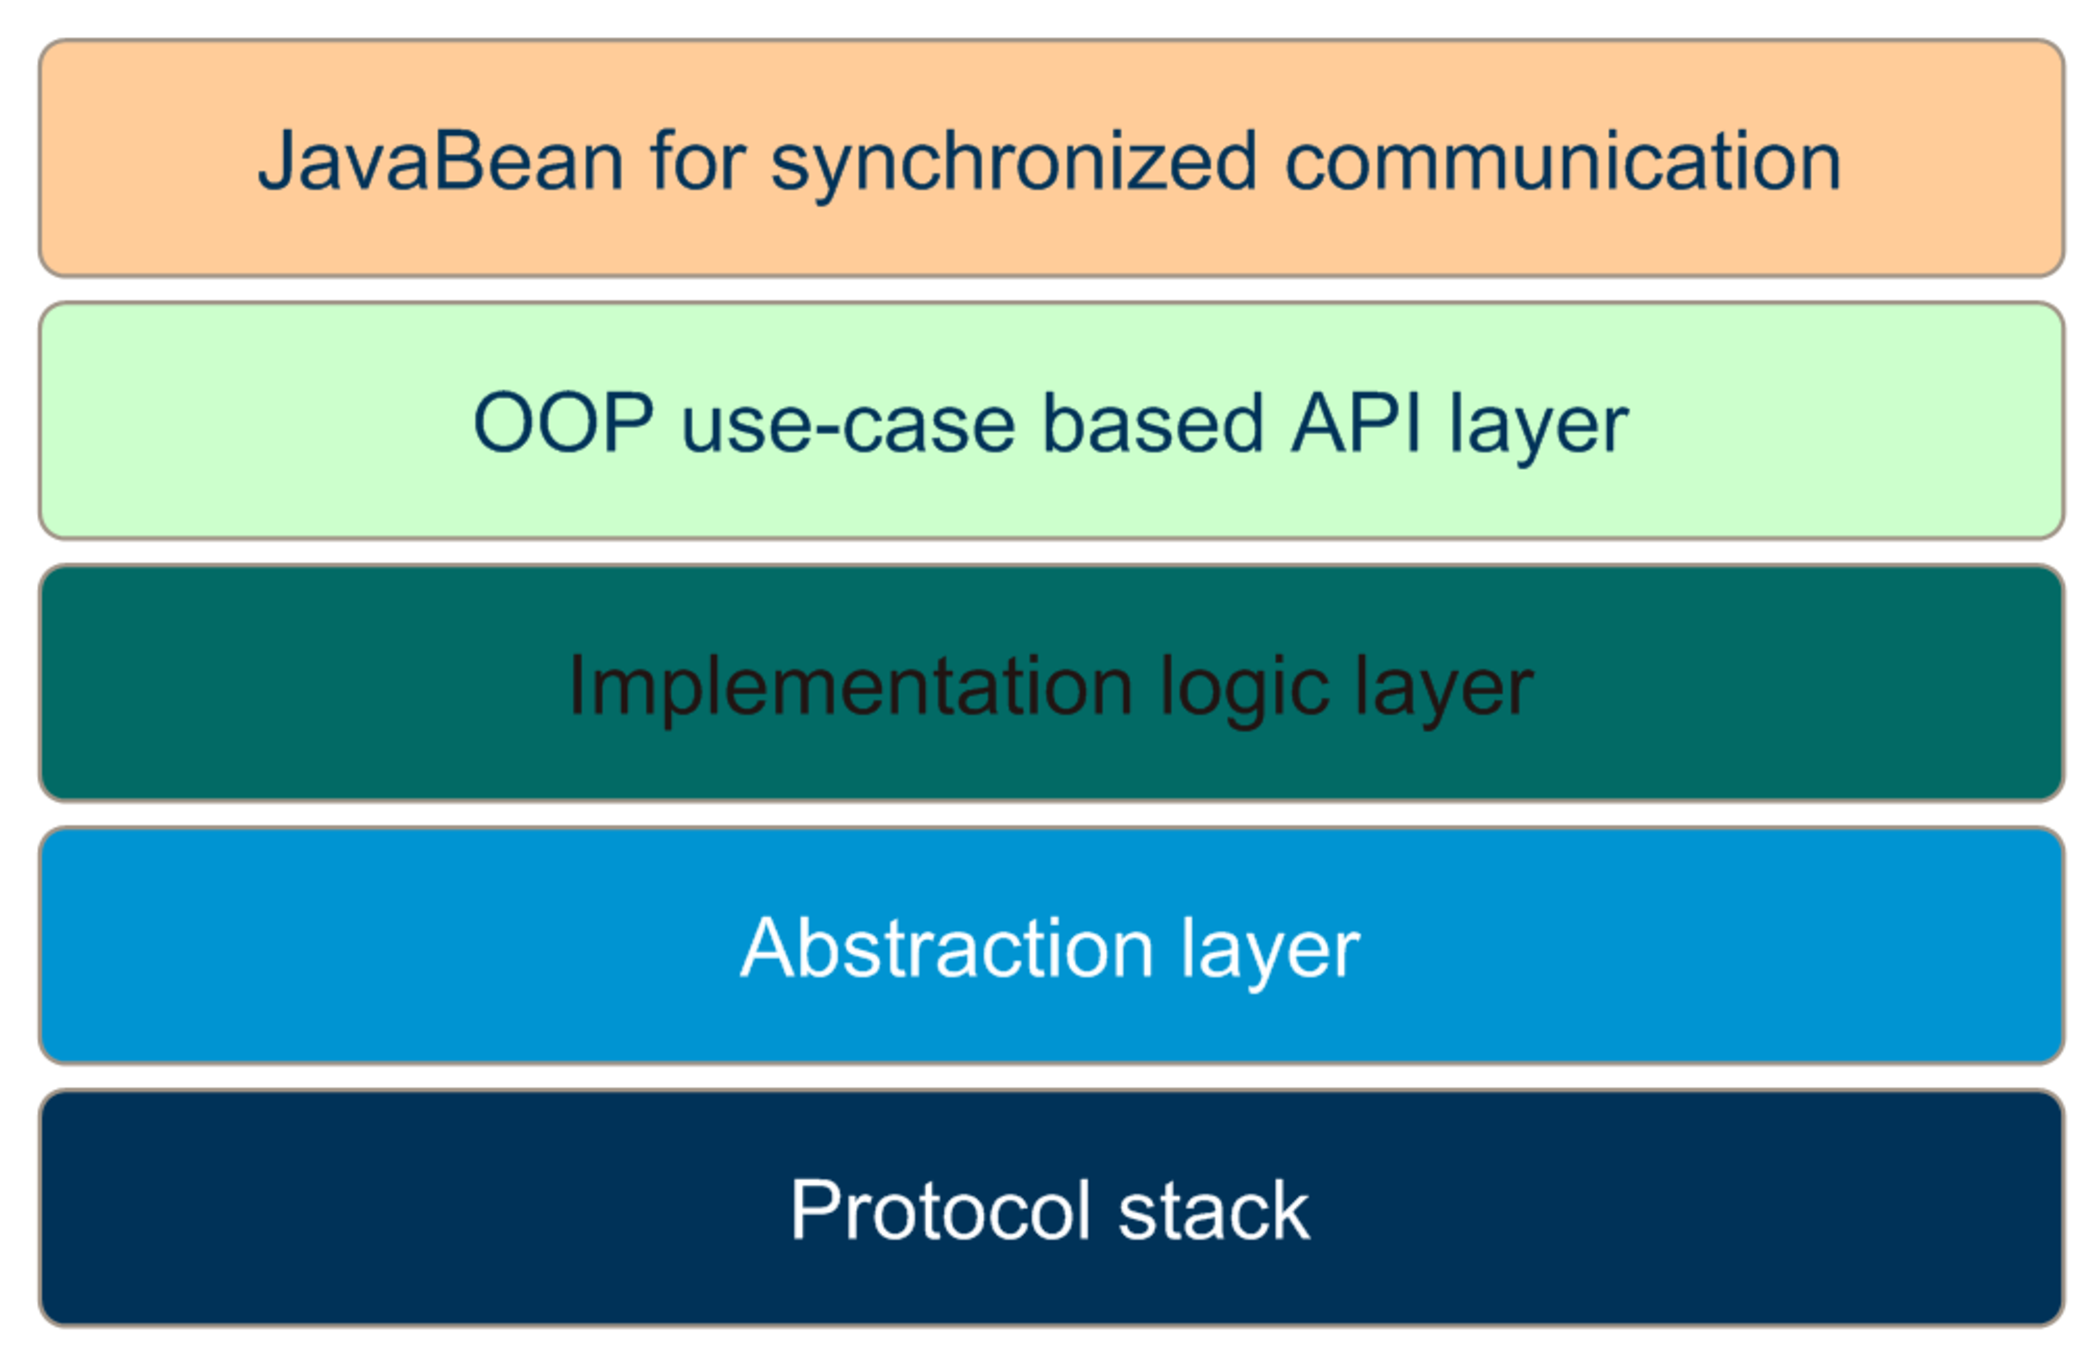
\epsfig{file=chap06/resources/five_layers, width=5.2in}
\caption{Five layers architecture}
\label{fig:FiveLayersArchitecture}
\end{figure}

\subsection{Protocol stack}

The protocol stack is the low level API for the project. There could be several implementations of the protocol stack. 

\subsection{Abstraction layer}

This layer is used for abstracting low level protocol stack. So the project can be easily migrated from one protocol stack to another without modifying the logic layer.

\subsection{Business logic layer}

This layer contains the main logic of the project.

\subsection{OOP use-case Based API Layer}

This layer is used for exposing public API for end user. Design Patterns such as Abstract Factory Pattern can be used here, especially for java SE.

\subsection{JavaBean for synchronized communication}

Components in Java are called beans. This layer contains the JavaBean which special designed for synchronized communication has two pairs of constructor and business logic group. The constructor which has the system parameters works with business logic which doesn't have system parameters. The constructor which doesn't have system parameters works with business logic which has the system parameters. In addition, this kind of JavaBean only has the method of \texttt{getState()} and no method of \texttt{setState()}. 

\section{Five layers architecture in Web Call Example Application}

Web Call Example Application follows the concept of five layers architecture. 

In SIP Call Component, there is abstraction layer and protocol stacks. As is shown in Figure \ref{fig:TheArchitectureOfSIPCallComponent}, among the four implementations of Third Party Call Controller, the three implementations on the left are based on \textsf{MjSIP} and Web Client is based on \textsf{Apache} \textsf{Common} \textsf{HttpClient}. An advantage of separate logic and Protocol stack is that users can choose to use different stacks according to their requirements. Another advantage is that developers can focus on the business logic part and no need to touch lower level stacks. In SIP Call Component, the abstraction layer defined a general interface for normal phone call behaviors, such as \texttt{start()} and \texttt{terminate()}. The interface of abstraction layer in SIP Call Component is shown in Figure \ref{fig:ClassDiagramOfSessionInterface}.  As the business logic of SIP Call Component, Call Controller only needs to take care of the call flow, e.g., set properties, register, make phone call and terminate call. And it will not handle any details about SIP message or media flow from the API level. The public API that opens to developers in SIP Call Component is the ``OOP use-case Based API Layer''. 

In Web Call Example Application, SIP Call Component is used as the base library of Web Application. However, it is designed to use as a standalone SIP call high level API. It is independent with other parts of the application. Any developers can take it and integrate it to their own applications.


\begin{figure}[!hbtp]
\centering
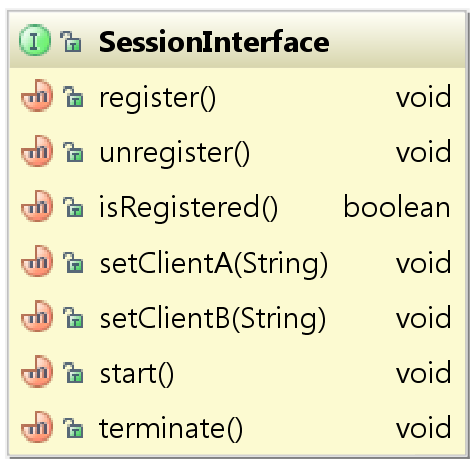
\epsfig{file=chap06/resources/SessionInterface_class_diagram, width=3in}
\caption{Class diagram of \texttt{SessionInterface}}
\label{fig:ClassDiagramOfSessionInterface}
\end{figure}



\section{Architecture of SIP Call Component}

The SIP Call Component is the core of Web Call Example Application. The design architecture is shown in Figure \ref{fig:TheArchitectureOfSIPCallComponent}.

\begin{figure}[!hbtp]
\centering
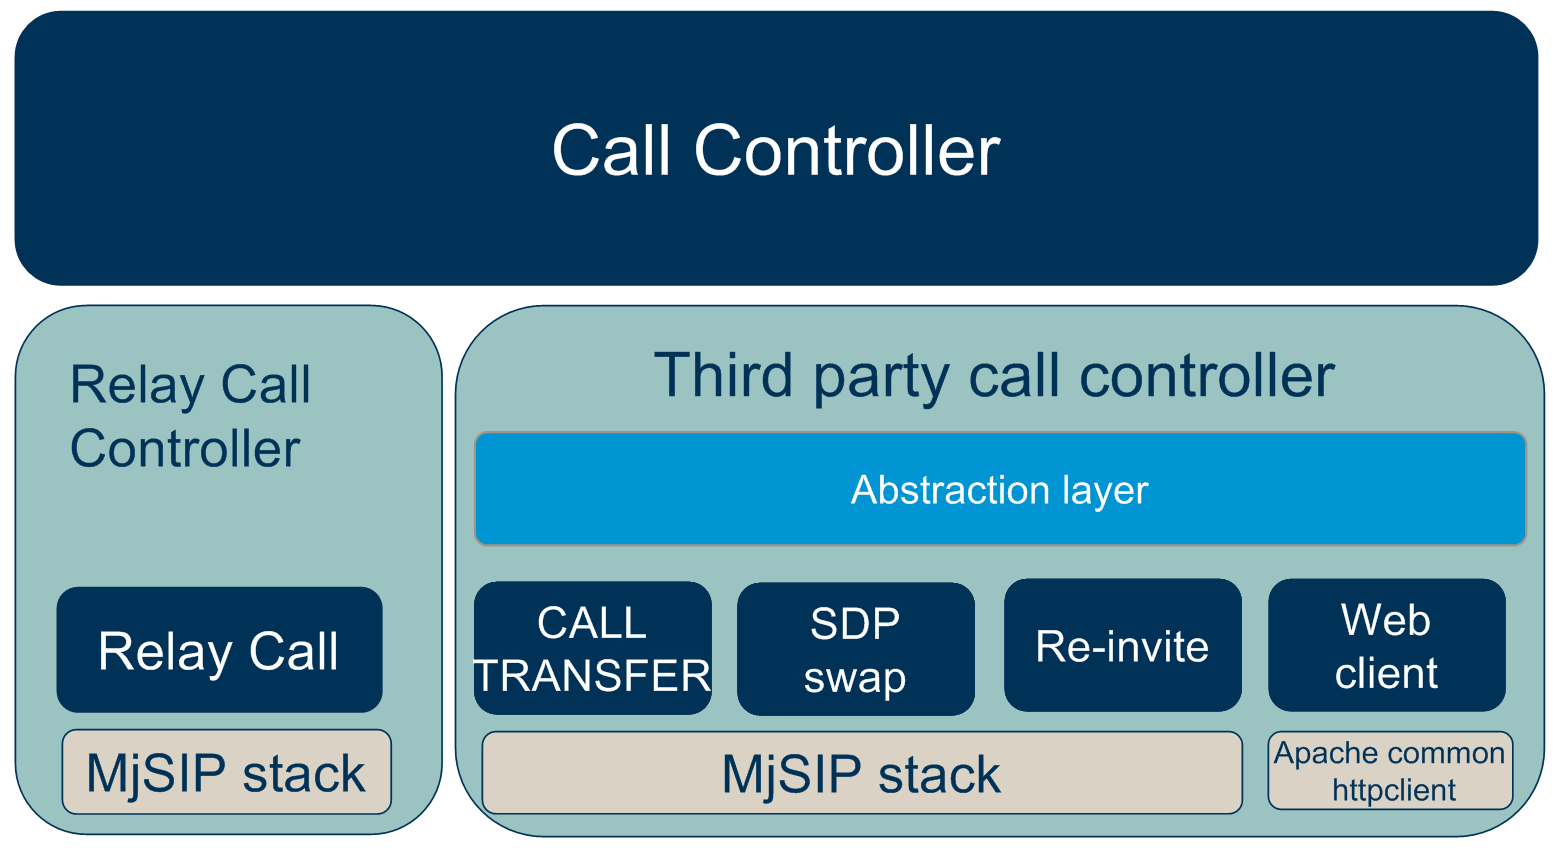
\epsfig{file=chap06/resources/sip_call_component_architecture, width=5.2in}
\caption{The Architecture of SIP Call Component}
\label{fig:TheArchitectureOfSIPCallComponent}
\end{figure}

It can be seen from Figure \ref{fig:TheArchitectureOfSIPCallComponent}, there is a interface \texttt{CallController} on the top of all kinds of call controllers. There are two subtype of Call Controller, one is Relay Call Controller and another is Third Party Call Controller. The Relay Call Controller is the legacy code of \textsf{Web Call SDK} which developed by Yuening Chen. In the old project, the Relay Call Controller is the core of all phone calls \cite{WebCallSDK}. However, in this version, four other implements are added to the SIP Call Component. They are Call Transfer, SDP Swap, Re-invite and Web Client. From a outside view, all the four methods are doing the same thing. They just try to establish a phone call between caller and callee. Chapter \ref{sec:Solution} describes the different among the four methods in detail. Chapter will focus on the architecture and design part. All four third party call methods are implemented the same interface. This means the user can easily switch call method from one to another. And other call method, if there is any, as long as it implements the interface at abstraction layer. It can be used in the SIP Call Component.

\section{Class Hierarchy}

The hierarchy of call controller is shown in Figure \ref{fig:CallControllerClassHierarchyDiagram}. All of call controllers are implemented the first interface \texttt{CallController}. This kind of design enables easily switch of call controllers. \texttt{SessionInterface} is an interface for third party call. \texttt{WebClientImpl}, \texttt{ReinviteImpl}, \texttt{SdpSwapImpl} and \texttt{MjSipCallTransferImpl} are implementations for \texttt{SessionInterface}. 

There are different call controller factories to create call controllers. The call controller factory follows the design pattern of \textsf{Abstract Factory}. An \textsf{Abstract Factory} is a class that exists to create instances of another class \cite{DesignPatternGoF}. The design of SIP Call Component considered that a call controller cannot only establish audio call, but also video call and message channels. This can be seen from the Figure \ref{fig:ControllerFactoryClassHierarchyDiagram}. The very general difference between Relay Call and Third Party Call is the way to handle media flow. But both of them should have the competence to establish all kind of sessions. In current version of Web Call Example Application, only audio call is implemented.

\begin{sidewaysfigure}
\centering
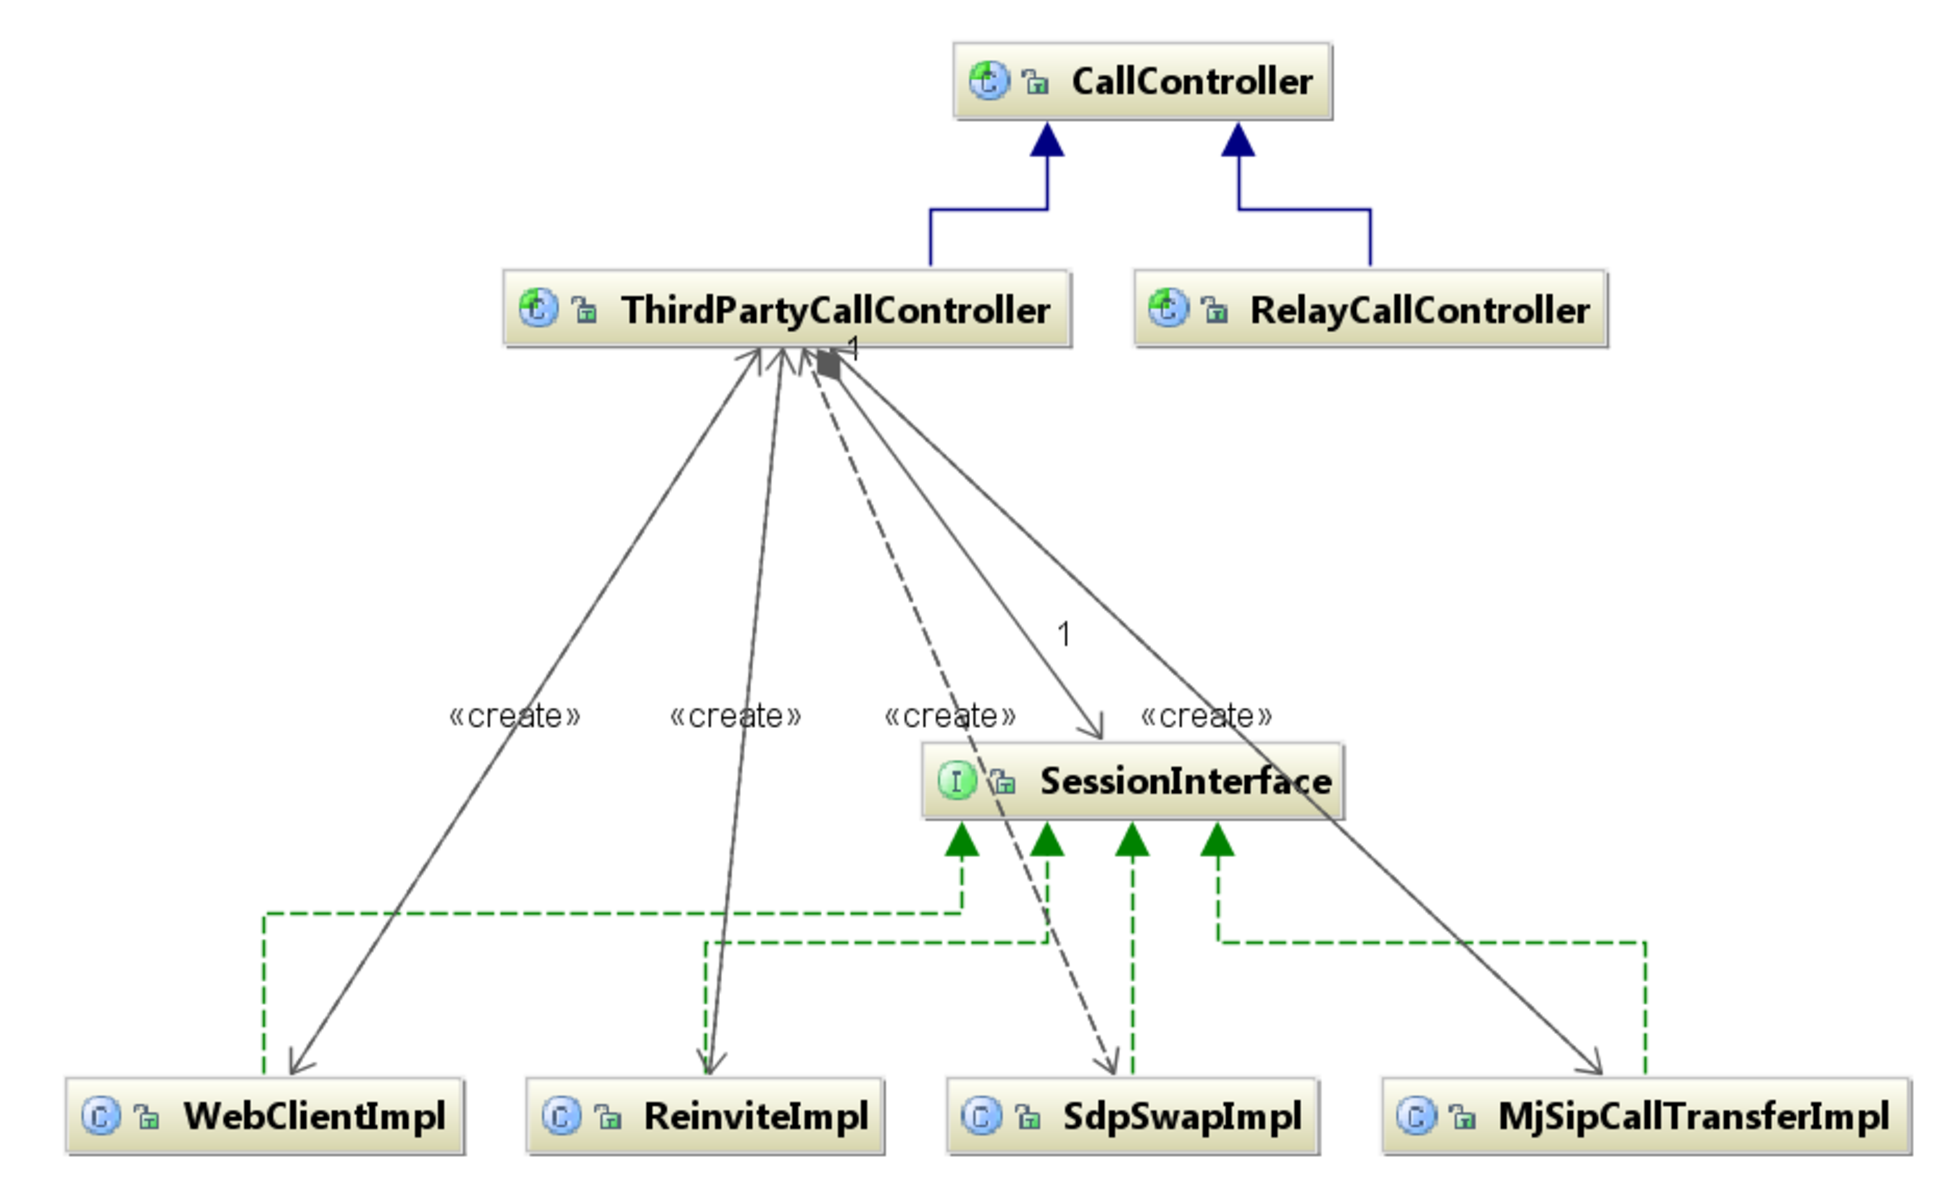
\epsfig{file=chap06/resources/call_controller_class_hierarchy_diagram,  width=8.3in}
\caption{Call Controller class hierarchy diagram}
\label{fig:CallControllerClassHierarchyDiagram}
\end{sidewaysfigure}

\begin{sidewaysfigure}
\centering
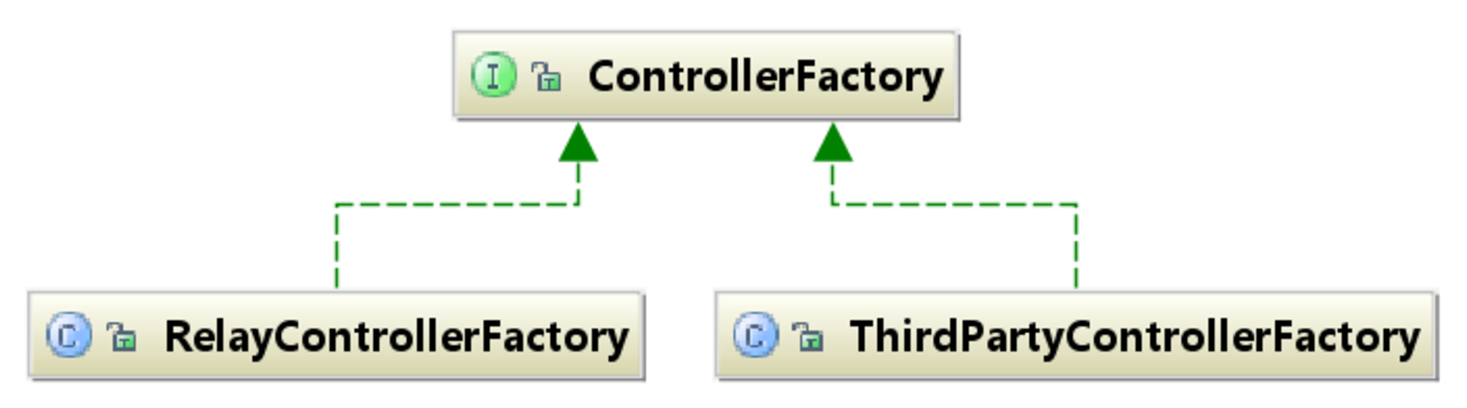
\epsfig{file=chap06/resources/factory_class_hierarchy_diagram, width=8.3in}
\caption{Controller Factory class hierarchy diagram}
\label{fig:ControllerFactoryClassHierarchyDiagram}
\end{sidewaysfigure}



% ********** End of chapter **********
